\begin{appendices}

\section{Visualization of generated images}\label{appendiximages}


\section{Posterior predictive distribution}\label{appendix1}
The posterior predictive distribution is given by:
\begin{align}
    p(f^*|x^*,\mathcal{D}) &= \int_{\Omega_{\bm{\theta}}}p(f^*,{\bm{\theta}}|x^*,\mathcal{D})d{\bm{\theta}}\\
    &=\int_{\Omega_{\bm{\theta}}}p(f^*|x^*,\mathcal{D},{\bm{\theta}})p({\bm{\theta}}|\mathcal{D})d{\bm{\theta}}\\
    &=\mathbb{E}_{{\bm{\theta}}\sim p({\bm{\theta}}|\mathcal{D})}\left[p(f^*|x^*,\mathcal{D},{\bm{\theta}})\right]\\
    &\approx N^{-1}\sum_{i=1}^N p(f^*|x^*,\mathcal{D}, {\bm{\theta}}^{(i)})
\end{align}
Where M denotes the number of samples, and:
\begin{equation}
    p(f^*|x^*,\mathcal{D}, {\bm{\theta}}^{(i)}) \sim \mathcal{N}\left(\mu_i^*, \, \, (\sigma_i^2)^*\right)
\end{equation}
Where: 
\begin{align*}
    &\mu_i^*=k_{{\bm{\theta}}^{(i)}}(S,x^*)^Tk_{{\bm{\theta}}^{(i)}}^{-1}y\\
    &(\sigma_i^2)^*=k_{{\bm{\theta}}^{(i)}}(x^*,x^*)-k_{{\bm{\theta}}^{(i)}}(S,x^*)^TK(S)^{-1}k_{{\bm{\theta}}^{(i)}}(S,x^*)
\end{align*}

\section{MCMC diagnostics for assessing mixing and required warm-up period}\label{appendix2}

\begin{figure}[H]
    \centering
    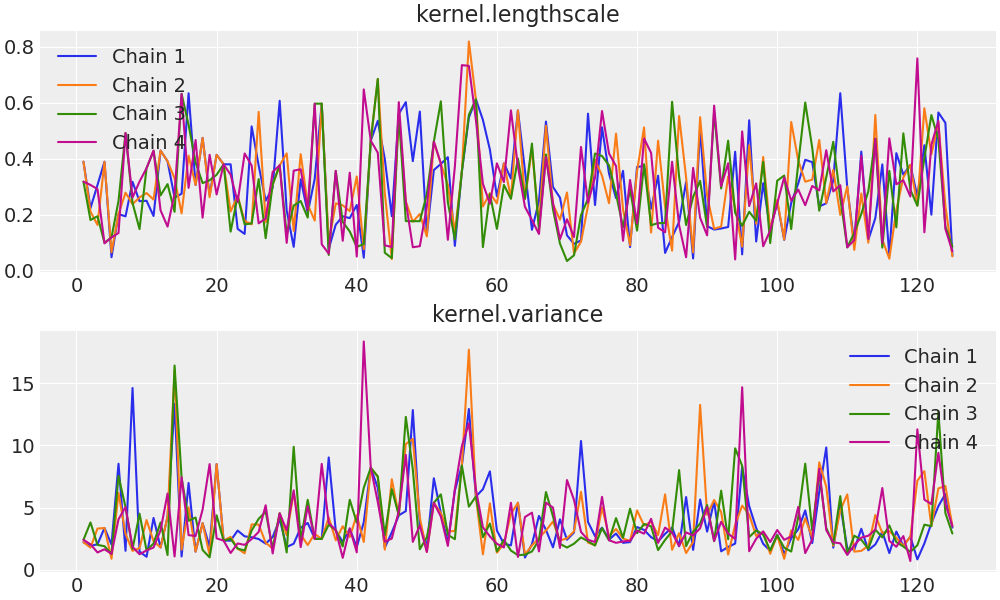
\includegraphics[width=0.5\textwidth]{src/traceplotsdiagnostics.png}
    \caption{Trace plots of the Markov chains with no warm-up period.}
    \label{fig:mcmcdiag}
\end{figure}

\begin{table}[H]
\centering
\resizebox{\textwidth}{!}{\begin{tabular}{lrrrrrrrrr}
\toprule
{} &   mean &     sd &  hdi\_2.5\% &  hdi\_97.5\% &  mcse\_mean &  mcse\_sd &  ess\_bulk &  ess\_tail &  r\_hat \\
\midrule
kernel.lengthscale &  0.296 &  0.157 &     0.043 &      0.596 &      0.012 &    0.009 &     167.0 &     169.0 &   1.04 \\
kernel.variance    &  3.820 &  2.698 &     0.706 &      8.632 &      0.232 &    0.165 &     154.0 &     228.0 &   1.03 \\
\bottomrule
\end{tabular}}
\caption[]{Diagnostics of MCMC samples generated by NUTS with no warm-up period.}
\label{tab:mcmcdiag}
\end{table}

\end{appendices}
